\documentclass[11pt]{article}
\usepackage[notes]{la}
\lamodule{2}{1}{Matrix Operations}
\laxdoc{1.4}
\laxdoc{1.8}
\laxdoc{1.9}

\begin{document}

\section{Matrix Operations}

\begin{guide}
Until now a matrix \emph{acted on vectors}: it was a machine $\bv{x}\mapsto A\bv{x}$ (Sections~1.4, 1.8 and 1.9). Now put two machines in a row: feed $\bv{x}$ to $B$, then feed the output to $A$. Is the result again a linear map, and if so, which matrix does it have? How is that matrix built from $A$ and $B$? Why should it matter which machine comes first? And what happens to a matrix if we exchange its rows and columns?
\end{guide}

\textbf{By the end of this section you should be able to:}
\begin{itemize}
  \item add and scale matrices, and say when the sizes allow it;
  \item explain why the matrix of ``first $B$, then $A$'' is the \emph{product} $AB$, and use that to define $AB$ column by column;
  \item compute a product by columns, by the row--column rule and by rows, and check its size before computing anything;
  \item find the matrix of a composite of plane maps by following $\bv{e}_1$ and $\bv{e}_2$, and by multiplying;
  \item explain, with examples, why $AB\neq BA$ in general, why $AB=\mathbf{0}$ does not force $A=\mathbf{0}$ or $B=\mathbf{0}$, and why $AB=AC$ does not force $B=C$;
  \item use the rules that \emph{do} hold: associativity, the two distributive laws, and $I A=A=AI$;
  \item compute powers $A^k$ and describe them geometrically for rotations, shears and stretches;
  \item define the transpose, and use $(AB)\T=B\T A\T$ with the sizes as a check.
\end{itemize}

% ---------------------------------------------------------------------
\subsection*{Adding and scaling matrices}

A matrix is a rectangular table of numbers, and two tables of the same shape can be added entry by entry, exactly as vectors are (Section~1.3).

\begin{defn}{Sum and scalar multiple}{sum}
Let $A$ and $B$ be $m\times n$ matrices with entries $a_{ij}$ and $b_{ij}$, and let $c$ be a scalar. The \emph{sum} $A+B$ is the $m\times n$ matrix with entries $a_{ij}+b_{ij}$, and the \emph{scalar multiple} $cA$ is the $m\times n$ matrix with entries $c\,a_{ij}$. The $m\times n$ \emph{zero matrix} $\mathbf{0}$ has every entry $0$. The sum of two matrices is defined \emph{only} when they have the same size.
\end{defn}

\begin{thm}{Rules for sums and scalar multiples}{addprops}
Let $A,B,C$ be matrices of the same size and let $r,s$ be scalars. Then
\begin{enumerate}[label=(\alph*),itemsep=1pt]
  \item $A+B=B+A$ and $(A+B)+C=A+(B+C)$;
  \item $A+\mathbf{0}=A$;
  \item $r(A+B)=rA+rB$ and $(r+s)A=rA+sA$;
  \item $r(sA)=(rs)A$.
\end{enumerate}
\end{thm}

\begin{proof}
Compare the $(i,j)$ entries on both sides. Each identity then says something about real numbers: $a_{ij}+b_{ij}=b_{ij}+a_{ij}$, $r(a_{ij}+b_{ij})=ra_{ij}+rb_{ij}$, and so on.
\end{proof}

\begin{exmp}{Sums and scalar multiples}{addex}
Let $A=\begin{bmatrix}4&0&5\\-1&3&2\end{bmatrix}$, \ $B=\begin{bmatrix}1&1&1\\3&5&7\end{bmatrix}$ and $C=\begin{bmatrix}2&-3\\0&1\end{bmatrix}$. Compute $A+B$, $2B$ and $A-2B$, and decide whether $A+C$ is defined.

\textbf{Solution.} $A$ and $B$ are both $2\times3$, so
\[
A+B=\begin{bmatrix}5&1&6\\2&8&9\end{bmatrix},\qquad
2B=\begin{bmatrix}2&2&2\\6&10&14\end{bmatrix},\qquad
A-2B=\begin{bmatrix}2&-2&3\\-7&-7&-12\end{bmatrix}.
\]
The matrix $C$ is $2\times2$ while $A$ is $2\times3$, so $A+C$ is \emph{not} defined: there is no entry of $C$ to pair with $a_{13}=5$.
\end{exmp}

\begin{kc}{Sizes for sums}{addsizes}
Let $P$ be $3\times2$, $Q$ be $3\times2$ and $R$ be $2\times3$. Which of $P+Q$, $P+R$, $3Q-P$ and $R-R$ are defined? What are their sizes?
\end{kc}

\begin{think}{Adding maps}{addmaps}
(a)~Show that $(A+B)\bv{x}=A\bv{x}+B\bv{x}$ for every $\bv{x}$, so the matrix $A+B$ is the matrix of the linear map $\bv{x}\mapsto A\bv{x}+B\bv{x}$. (b)~Is the map $\bv{x}\mapsto A\bv{x}+B\bv{x}$ the same thing as the composite ``first $B$, then $A$''? Test with $A=B=I$.
\end{think}

% ---------------------------------------------------------------------
\subsection*{Doing one map after another: the product}

Let $B$ be an $n\times p$ matrix and $A$ an $m\times n$ matrix. Then $\bv{x}\mapsto B\bv{x}$ sends $\R^p$ to $\R^n$, and $\bv{y}\mapsto A\bv{y}$ sends $\R^n$ to $\R^m$. Feeding the output of the first into the second gives the composite
\[
\bv{x}\ \longmapsto\ B\bv{x}\ \longmapsto\ A(B\bv{x}),\qquad \R^p\to\R^n\to\R^m .
\]
This composite is linear: by Theorem~\ref{1.4-thm:linear}, $A(B(\bv{u}+\bv{v}))=A(B\bv{u}+B\bv{v})=A(B\bv{u})+A(B\bv{v})$ and $A(B(c\bv{u}))=A(cB\bv{u})=cA(B\bv{u})$. So by Theorem~\ref{1.9-thm:stdthm} it has a \emph{unique} standard matrix, whose $j$th column is the image of $\bv{e}_j$. Follow $\bv{e}_j$ through both steps: $B\bv{e}_j=\bv{b}_j$ is the $j$th column of $B$ (Example~\ref{1.4-ex:ei}), and then $A$ is applied to it. So the $j$th column of the matrix of the composite is $A\bv{b}_j$. We take this as the definition.

\begin{defn}{The product $AB$}{product}
Let $A$ be an $m\times n$ matrix and $B$ an $n\times p$ matrix with columns $\bv{b}_1,\dots,\bv{b}_p$. The \emph{product} $AB$ is the $m\times p$ matrix whose columns are $A\bv{b}_1,\dots,A\bv{b}_p$:
\[
AB=A\begin{bmatrix}\bv{b}_1&\bv{b}_2&\cdots&\bv{b}_p\end{bmatrix}=\begin{bmatrix}A\bv{b}_1&A\bv{b}_2&\cdots&A\bv{b}_p\end{bmatrix}.
\]
\end{defn}

\begin{thm}{The product is the composite}{composite}
For $A$ of size $m\times n$, $B$ of size $n\times p$ and every $\bv{x}$ in $\R^p$,
\[
A(B\bv{x})=(AB)\bv{x}.
\]
In words: the matrix of ``first $B$, then $A$'' is $AB$. The factors are written in the order opposite to the order in which the steps happen, like the functions $f(g(x))$.
\end{thm}

\begin{proof}
Write $B\bv{x}=x_1\bv{b}_1+\cdots+x_p\bv{b}_p$ (Definition~\ref{1.4-def:matvec}). Linearity of $A$ (Theorem~\ref{1.8-thm:props}(c)) gives
\[
A(B\bv{x})=x_1A\bv{b}_1+\cdots+x_pA\bv{b}_p=\begin{bmatrix}A\bv{b}_1&\cdots&A\bv{b}_p\end{bmatrix}\bv{x}=(AB)\bv{x}.
\]
\end{proof}

Here is the picture for the plane, following $\bv{e}_1$ and $\bv{e}_2$ as in Section~1.9. Take $B$ to be the rotation by $90^\circ$ and $A$ the shear $\begin{bmatrix}1&2\\0&1\end{bmatrix}$.

\begin{center}
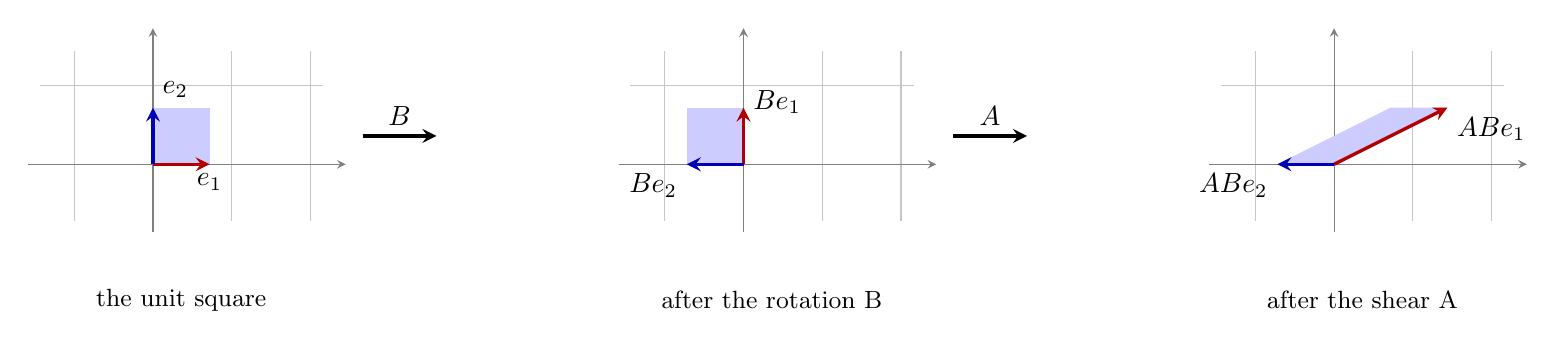
\begin{tikzpicture}[x=0.72cm,y=0.72cm,>=stealth]
  \draw[gray!45] (-2,-1) grid (3,2);
  \draw[->,gray] (-2.2,0)--(3.4,0); \draw[->,gray] (0,-1.2)--(0,2.4);
  \fill[blue!20] (0,0) rectangle (1,1);
  \draw[->,very thick,red!70!black] (0,0)--(1,0);
  \draw[->,very thick,blue!70!black] (0,0)--(0,1);
  \node[below] at (1,0) {$e_1$};
  \node[above right] at (0,1) {$e_2$};
  \node at (0.5,-2.4) {\small the unit square};
  \draw[->,very thick] (3.7,0.5)--(5.0,0.5) node[midway,above] {$B$};
  \begin{scope}[xshift=7.5cm]
    \draw[gray!45] (-2,-1) grid (3,2);
    \draw[->,gray] (-2.2,0)--(3.4,0); \draw[->,gray] (0,-1.2)--(0,2.4);
    \fill[blue!20] (0,0)--(0,1)--(-1,1)--(-1,0)--cycle;
    \draw[->,very thick,red!70!black] (0,0)--(0,1);
    \draw[->,very thick,blue!70!black] (0,0)--(-1,0);
    \node[right] at (0,1.1) {$Be_1$};
    \node[below left] at (-1,0) {$Be_2$};
    \node at (0.5,-2.4) {\small after the rotation B};
    \draw[->,very thick] (3.7,0.5)--(5.0,0.5) node[midway,above] {$A$};
  \end{scope}
  \begin{scope}[xshift=15cm]
    \draw[gray!45] (-2,-1) grid (3,2);
    \draw[->,gray] (-2.2,0)--(3.4,0); \draw[->,gray] (0,-1.2)--(0,2.4);
    \fill[blue!20] (0,0)--(2,1)--(1,1)--(-1,0)--cycle;
    \draw[->,very thick,red!70!black] (0,0)--(2,1);
    \draw[->,very thick,blue!70!black] (0,0)--(-1,0);
    \node[below right] at (2,1) {$ABe_1$};
    \node[below left] at (-1,0) {$ABe_2$};
    \node at (0.5,-2.4) {\small after the shear A};
  \end{scope}
\end{tikzpicture}
\end{center}

\textbf{Figure.} Two steps. The rotation $B$ takes $\bv{e}_1$ to $(0,1)$ and $\bv{e}_2$ to $(-1,0)$. The shear $A$ then takes $(0,1)$ to $(2,1)$ and leaves $(-1,0)$ where it is. The columns of the composite are therefore $(2,1)$ and $(-1,0)$: $AB=\begin{bmatrix}2&-1\\1&0\end{bmatrix}$, which is the answer to the first question at the end of Section~1.9. The unit square has become the slanted parallelogram in the last panel.

\begin{warn}[Sizes must match]
$AB$ is defined only when the number of \emph{columns} of $A$ equals the number of \emph{rows} of $B$: an $m\times n$ matrix times an $n\times p$ matrix is an $m\times p$ matrix. The reason is the composite: $B$ delivers vectors of $\R^n$, and $A$ can only accept vectors of $\R^n$. Always write the sizes first, $(m\times n)(n\times p)\to m\times p$, and look at the two inner numbers.
\end{warn}

\begin{exmp}{A product, column by column}{prodcols}
Let $A=\begin{bmatrix}1&2&0\\-1&1&3\end{bmatrix}$ ($2\times3$) and $B=\begin{bmatrix}2&1\\0&-1\\1&4\end{bmatrix}$ ($3\times2$). Compute $AB$ and $BA$.

\textbf{Solution.} The inner sizes agree in $AB$, so $AB$ is $2\times2$. Its columns are $A$ times the columns of $B$:
\[
A\begin{bmatrix}2\\0\\1\end{bmatrix}=2\begin{bmatrix}1\\-1\end{bmatrix}+0\begin{bmatrix}2\\1\end{bmatrix}+1\begin{bmatrix}0\\3\end{bmatrix}=\begin{bmatrix}2\\1\end{bmatrix},\qquad
A\begin{bmatrix}1\\-1\\4\end{bmatrix}=\begin{bmatrix}1\\-1\end{bmatrix}-\begin{bmatrix}2\\1\end{bmatrix}+4\begin{bmatrix}0\\3\end{bmatrix}=\begin{bmatrix}-1\\10\end{bmatrix}.
\]
So $AB=\begin{bmatrix}2&-1\\1&10\end{bmatrix}$. The product $BA$ is also defined, because $B$ is $3\times2$ and $A$ is $2\times3$; but it is a $3\times3$ matrix,
\[
BA=\begin{bmatrix}1&5&3\\1&-1&-3\\-3&6&12\end{bmatrix},
\]
which has nothing in common with $AB$ except the letters. Not even the sizes agree.
\end{exmp}

\subsection*{The row--column rule}

By hand it is faster to compute one entry at a time. The $(i,j)$ entry of $AB$ is the $i$th entry of the $j$th column $A\bv{b}_j$, and by the row--column rule for $A\bv{x}$ (Theorem~\ref{1.4-thm:rowcol}) that entry is a sum of products.

\begin{thm}{The row--column rule for $AB$}{rowcol}
If $A$ is $m\times n$ and $B$ is $n\times p$, then
\[
(AB)_{ij}=a_{i1}b_{1j}+a_{i2}b_{2j}+\cdots+a_{in}b_{nj},
\]
the sum of the products of the entries of row $i$ of $A$ with the corresponding entries of column $j$ of $B$.
\end{thm}

\begin{center}
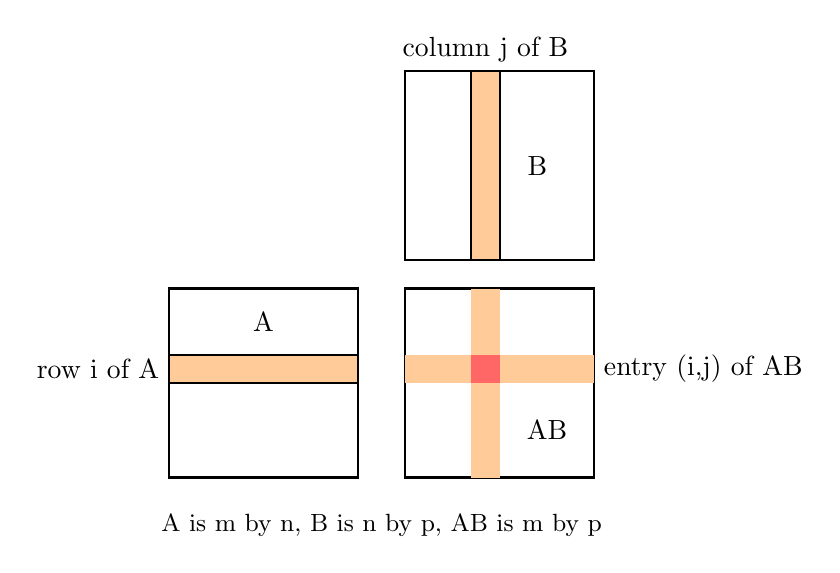
\begin{tikzpicture}[x=0.6cm,y=0.6cm,>=stealth]
  \draw[thick] (0,0) rectangle (4,4);
  \draw[thick] (5,4.6) rectangle (9,8.6);
  \draw[thick] (5,0) rectangle (9,4);
  \fill[orange!40] (0,2) rectangle (4,2.6);
  \fill[orange!40] (6.4,4.6) rectangle (7,8.6);
  \fill[orange!40] (5,2) rectangle (9,2.6);
  \fill[orange!40] (6.4,0) rectangle (7,4);
  \fill[red!60] (6.4,2) rectangle (7,2.6);
  \draw[thick] (0,2) rectangle (4,2.6);
  \draw[thick] (6.4,4.6) rectangle (7,8.6);
  \node at (2,3.3) {A};
  \node at (7.8,6.6) {B};
  \node at (8.0,1.0) {AB};
  \node[left] at (0,2.3) {row i of A};
  \node[above] at (6.7,8.6) {column j of B};
  \node[right] at (9,2.3) {entry (i,j) of AB};
  \node at (4.5,-1.0) {\small A is m by n, B is n by p, AB is m by p};
\end{tikzpicture}
\end{center}

\textbf{Figure.} To fill the entry of $AB$ in row $i$ and column $j$ (the red square), run along row $i$ of $A$ and down column $j$ of $B$ at the same time, multiply the pairs and add. That is why a row of $A$ and a column of $B$ must have the same length $n$.

\begin{proc}{Computing a product $AB$}{product}
\begin{enumerate}
  \item Write the sizes $(m\times n)(n\times p)$. If the inner numbers differ, $AB$ is not defined. Otherwise $AB$ is $m\times p$.
  \item Compute each column $A\bv{b}_j$ (a combination of the columns of $A$), or each entry with the row--column rule.
  \item Check: choose a vector $\bv{x}$ in $\R^p$ and compare $(AB)\bv{x}$ with $A(B\bv{x})$ (Theorem~\ref{thm:composite}).
\end{enumerate}
\end{proc}

\begin{exmp}{The same product by the row--column rule}{rowcol}
For $A$ and $B$ of Example~\ref{ex:prodcols}, the entry in row $2$ and column $2$ of $AB$ pairs row $2$ of $A$, namely $\begin{bmatrix}-1&1&3\end{bmatrix}$, with column $2$ of $B$, namely $(1,-1,4)$:
\[
(AB)_{22}=(-1)(1)+(1)(-1)+(3)(4)=-1-1+12=10,
\]
agreeing with the second column found there. The entry $(AB)_{12}=(1)(1)+(2)(-1)+(0)(4)=-1$. Now the check of step~3 with $\bv{x}=(1,2)$: $B\bv{x}=(4,-2,9)$ and $A(B\bv{x})=(4-4+0,\ -4-2+27)=(0,21)$; and $(AB)\bv{x}=(2-2,\ 1+20)=(0,21)$. \ $\checkmark$
\end{exmp}

\begin{exmp}{Rotate, then shear}{planeprod}
Let $B=\begin{bmatrix}0&-1\\1&0\end{bmatrix}$ be the rotation by $90^\circ$ and $A=\begin{bmatrix}1&2\\0&1\end{bmatrix}$ the shear of the figure. The matrix of ``first $B$, then $A$'' is
\[
AB=\begin{bmatrix}A\begin{bmatrix}0\\1\end{bmatrix}&A\begin{bmatrix}-1\\0\end{bmatrix}\end{bmatrix}=\begin{bmatrix}2&-1\\1&0\end{bmatrix},
\]
the same matrix we found by following $\bv{e}_1$ and $\bv{e}_2$. By the row--column rule: row $1$ of $A$ with column $1$ of $B$ gives $1\cdot0+2\cdot1=2$, row $1$ with column $2$ gives $1\cdot(-1)+2\cdot0=-1$, row $2$ with column $1$ gives $0\cdot0+1\cdot1=1$, and row $2$ with column $2$ gives $0$. The composite sends $(1,1)$ to $(1,1)$: indeed $B(1,1)=(-1,1)$ and then $A(-1,1)=(-1+2,\ 1)=(1,1)$.
\end{exmp}

\begin{kc}{Is it defined? How big is it?}{prodsizes}
Let $A$ be $2\times4$, $B$ be $4\times3$, $C$ be $3\times2$. Which of $AB$, $BA$, $BC$, $CA$, $AC$ and $ABC$ are defined? Give the size of each that is.
\end{kc}

\begin{kc}{Compute}{prodcompute}
Let $A=\begin{bmatrix}1&-2\\3&0\end{bmatrix}$ and $B=\begin{bmatrix}2&1&0\\-1&4&3\end{bmatrix}$. Compute $AB$ by columns, check one entry by the row--column rule, and say whether $BA$ is defined.
\end{kc}

\begin{think}{Why must the sizes match?}{sizes}
(a)~Use the picture of a composite to explain in one sentence why $AB$ requires the \emph{columns} of $A$ to match the \emph{rows} of $B$, and not, say, the rows of $A$ to match the rows of $B$. (b)~If $A$ is $3\times5$ and $AB$ is $3\times7$, what is the size of $B$? (c)~If $AB$ and $BA$ are both defined, what can you say about the sizes of $A$ and $B$?
\end{think}

% ---------------------------------------------------------------------
\subsection*{Columns and rows of a product}

Definition~\ref{def:product} says that every column of $AB$ is a combination of the columns of $A$, with weights taken from the corresponding column of $B$. The same idea works for rows.

\begin{thm}{Rows of a product}{rowview}
The $i$th row of $AB$ equals $(\text{row } i \text{ of } A)\,B$. Equivalently, row $i$ of $AB$ is the combination
\[
a_{i1}\,(\text{row }1\text{ of }B)+a_{i2}\,(\text{row }2\text{ of }B)+\cdots+a_{in}\,(\text{row }n\text{ of }B).
\]
\end{thm}

\begin{proof}
The $j$th entry of row $i$ of $AB$ is $\sum_k a_{ik}b_{kj}$ (Theorem~\ref{thm:rowcol}). The $j$th entry of $a_{i1}(\text{row }1\text{ of }B)+\cdots+a_{in}(\text{row }n\text{ of }B)$ is $a_{i1}b_{1j}+\cdots+a_{in}b_{nj}$, the same sum.
\end{proof}

So: \emph{columns of $AB$ are combinations of the columns of $A$}, and \emph{rows of $AB$ are combinations of the rows of $B$}. Which of the two descriptions to use depends on the question.

\begin{exmp}{A single row of a product}{rowview}
For the matrices of Example~\ref{ex:prodcols}, row $2$ of $AB$ is row $2$ of $A$ times $B$:
\[
\begin{bmatrix}-1&1&3\end{bmatrix}\begin{bmatrix}2&1\\0&-1\\1&4\end{bmatrix}=-1\begin{bmatrix}2&1\end{bmatrix}+1\begin{bmatrix}0&-1\end{bmatrix}+3\begin{bmatrix}1&4\end{bmatrix}=\begin{bmatrix}-2&-1\end{bmatrix}+\begin{bmatrix}0&-1\end{bmatrix}+\begin{bmatrix}3&12\end{bmatrix}=\begin{bmatrix}1&10\end{bmatrix},
\]
which is the second row $\begin{bmatrix}1&10\end{bmatrix}$ of $AB=\begin{bmatrix}2&-1\\1&10\end{bmatrix}$. We computed one row without computing the rest.
\end{exmp}

\begin{exmp}{Scaling rows and scaling columns}{diag}
Let $D=\begin{bmatrix}2&0\\0&3\end{bmatrix}$ and $A=\begin{bmatrix}1&2\\3&4\end{bmatrix}$. Compare $DA$ and $AD$.

\textbf{Solution.} Rows of $DA$ are combinations of the rows of $A$ with weights from the rows of $D$: row $1$ is $2\,(\text{row }1\text{ of }A)$ and row $2$ is $3\,(\text{row }2\text{ of }A)$. So
\[
DA=\begin{bmatrix}2&4\\9&12\end{bmatrix}.
\]
Columns of $AD$ are combinations of the columns of $A$ with weights from the columns of $D$: column $1$ is $2\,(\text{column }1\text{ of }A)$ and column $2$ is $3\,(\text{column }2\text{ of }A)$. So
\[
AD=\begin{bmatrix}2&6\\6&12\end{bmatrix}.
\]
Multiplying by a diagonal matrix on the \emph{left} scales the \emph{rows}; on the \emph{right} it scales the \emph{columns}. The two products are different matrices.
\end{exmp}

\begin{kc}{Left or right?}{scaling}
Let $D=\begin{bmatrix}3&0\\0&1\end{bmatrix}$ and $A=\begin{bmatrix}2&1\\0&5\end{bmatrix}$. Without multiplying row by column, write $DA$ and $AD$, and say which entry of $A$ is affected by $D$ in each case.
\end{kc}

\begin{think}{Rows or columns?}{rowscols}
(a)~In Example~\ref{ex:diag}, which matrix would you multiply by on the left, and which on the right, to \emph{double column~2} of $A$ and leave column~1 alone? To \emph{add three times row~1 to row~2}? (b)~For $AB$, which of the following can be read off from the columns of $A$ alone: the range of the map $\bv{x}\mapsto AB\bv{x}$ (Definition~\ref{1.8-def:mattrans}) or the rows of $AB$? Why?
\end{think}

% ---------------------------------------------------------------------
\subsection*{Order matters}

Ask a question you would never ask about numbers: does $AB=BA$? Section~1.9 already gave the answer for plane maps (``order matters''), and the product turns that observation into a computation.

\begin{exmp}{Rotate then reflect, reflect then rotate}{order}
Let $R=\begin{bmatrix}0&-1\\1&0\end{bmatrix}$ be the rotation by $90^\circ$ and $F=\begin{bmatrix}1&0\\0&-1\end{bmatrix}$ the reflection in the $x_1$-axis. Compute $FR$ (first $R$, then $F$) and $RF$ (first $F$, then $R$).

\textbf{Solution.} Columns of $FR$ are $F$ times the columns of $R$, which are $(0,1)$ and $(-1,0)$:
\[
FR=\begin{bmatrix}F\begin{bmatrix}0\\1\end{bmatrix}&F\begin{bmatrix}-1\\0\end{bmatrix}\end{bmatrix}=\begin{bmatrix}0&-1\\-1&0\end{bmatrix}.
\]
Columns of $RF$ are $R$ times the columns of $F$, which are $(1,0)$ and $(0,-1)$:
\[
RF=\begin{bmatrix}R\begin{bmatrix}1\\0\end{bmatrix}&R\begin{bmatrix}0\\-1\end{bmatrix}\end{bmatrix}=\begin{bmatrix}0&1\\1&0\end{bmatrix}.
\]
So $FR\neq RF$. Geometrically $FR$ is the reflection in the line $x_2=-x_1$ and $RF$ is the reflection in the line $x_2=x_1$; the picture shows an asymmetric figure, the L-shape of Section~1.9, being sent to two different places.
\end{exmp}

\begin{center}
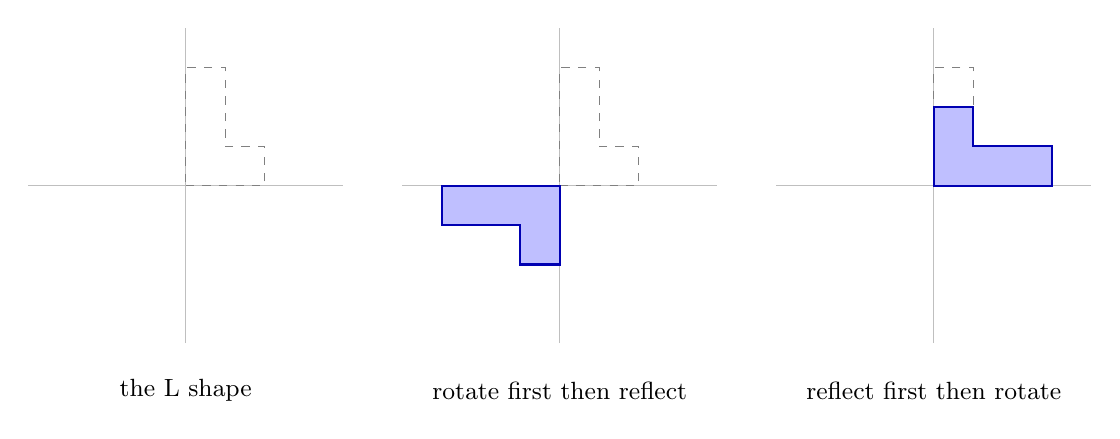
\begin{tikzpicture}[x=0.5cm,y=0.5cm,>=stealth]
  \foreach \cx in {0,9.5,19}{
    \begin{scope}[shift={(\cx,0)}]
      \draw[gray!50] (-4,0)--(4,0); \draw[gray!50] (0,-4)--(0,4);
      \draw[dashed,gray] (0,0)--(2,0)--(2,1)--(1,1)--(1,3)--(0,3)--cycle;
    \end{scope}}
  \begin{scope}[xshift=0cm]
    \node at (0,-5.2) {\small the L shape};
  \end{scope}
  \begin{scope}[shift={(9.5,0)}]
    \draw[thick,blue!70!black,fill=blue!25] (0,0)--(0,-2)--(-1,-2)--(-1,-1)--(-3,-1)--(-3,0)--cycle;
    \node at (0,-5.2) {\small rotate first then reflect};
  \end{scope}
  \begin{scope}[shift={(19,0)}]
    \draw[thick,blue!70!black,fill=blue!25] (0,0)--(0,2)--(1,2)--(1,1)--(3,1)--(3,0)--cycle;
    \node at (0,-5.2) {\small reflect first then rotate};
  \end{scope}
\end{tikzpicture}
\end{center}

\textbf{Figure.} The dashed L is the same in each panel. Middle: rotate by $90^\circ$ and then reflect in the $x_1$-axis, the matrix $FR$. Right: reflect and then rotate, the matrix $RF$. The two results are mirror images of each other across the line $x_2=-x_1$, but they are different sets.

There are three separate ways in which $AB$ can differ from $BA$. (1)~$AB$ may be defined while $BA$ is not. (2)~Both may be defined but have different \emph{sizes} (Example~\ref{ex:prodcols}). (3)~Both may have the same size and still be different matrices (Example~\ref{ex:order}). Only in rare cases are they equal; we then say $A$ and $B$ \emph{commute}.

\begin{exmp}{Cancellation fails and zero products}{zerodiv}
Let $A=\begin{bmatrix}1&1\\1&1\end{bmatrix}$, \ $B=\begin{bmatrix}2&0\\0&1\end{bmatrix}$ and $C=\begin{bmatrix}1&1\\1&0\end{bmatrix}$.

\textbf{(a)} Then
\[
AB=\begin{bmatrix}2&1\\2&1\end{bmatrix}=AC,\qquad\text{although } B\neq C.
\]
So $AB=AC$ does not allow us to ``cancel $A$''. Look at the difference: $A(B-C)=\mathbf{0}$ with $B-C=\begin{bmatrix}1&-1\\-1&1\end{bmatrix}\neq\mathbf{0}$.

\textbf{(b)} The same example shows that a product can be the zero matrix when neither factor is: $A(B-C)=\begin{bmatrix}1&1\\1&1\end{bmatrix}\begin{bmatrix}1&-1\\-1&1\end{bmatrix}=\begin{bmatrix}0&0\\0&0\end{bmatrix}$.

\textbf{(c)} \emph{Why?} The map $\bv{x}\mapsto A\bv{x}=(x_1+x_2)(1,1)$ crushes the whole plane onto the line spanned by $(1,1)$ (compare the projection in Section~1.8, and Theorem~\ref{1.9-thm:ontoone}). The columns of $B-C$ are multiples of $(1,-1)$, and every multiple of $(1,-1)$ is sent to $\bv{0}$. Two inputs that differ by a multiple of $(1,-1)$ share an output (Theorem~\ref{1.8-thm:sameimage}), so $A$ cannot tell $B\bv{x}$ from $C\bv{x}$ when they differ in that direction.
\end{exmp}

\begin{warn}[Matrices are not numbers]
For matrices \emph{in general}: $AB\neq BA$; from $AB=AC$ you may \emph{not} conclude $B=C$; from $AB=\mathbf{0}$ you may \emph{not} conclude $A=\mathbf{0}$ or $B=\mathbf{0}$; and $(A+B)^2\neq A^2+2AB+B^2$. Every familiar identity that silently uses $ab=ba$ has to be re-examined.
\end{warn}

\begin{kc}{Does order matter here?}{order}
Let $A=\begin{bmatrix}1&1\\0&1\end{bmatrix}$ (a horizontal shear) and $B=\begin{bmatrix}1&0\\1&1\end{bmatrix}$ (a vertical shear). Compute $AB$ and $BA$. Test both on $\bv{e}_1$ and say what each composite does to it.
\end{kc}

\begin{kc}{Expanding a product}{expand}
Let $A=\begin{bmatrix}1&2\\3&4\end{bmatrix}$ and $B=\begin{bmatrix}0&1\\1&0\end{bmatrix}$. (a)~Compute $(A+B)(A-B)$. (b)~Compute $A^2-B^2$. (c)~Expand $(A+B)(A-B)$ using the distributive laws, \emph{without} commuting any factors, and explain the discrepancy.
\end{kc}

\begin{think}{Who commutes?}{commute}
Decide, with a reason, whether the order matters for each pair. (a)~Two rotations of the plane. (b)~$A$ and $I$. (c)~Two diagonal $2\times2$ matrices. (d)~A matrix $A$ and $A^2=AA$. (e)~The projection onto the $x_1$-axis and the projection onto the $x_2$-axis. What do the pairs that commute have in common, geometrically or algebraically?
\end{think}

% ---------------------------------------------------------------------
\subsection*{The rules that do hold}

Order matters for the factors, but nothing else in the arithmetic is lost.

\begin{thm}{Algebra of the product}{mulprops}
Let $A$ be $m\times n$ and let $B$ and $C$ have the sizes that make each expression defined. Then, for every scalar $r$,
\begin{enumerate}[label=(\alph*),itemsep=1pt]
  \item $A(BC)=(AB)C$ \quad (associative law);
  \item $A(B+C)=AB+AC$ \quad and \quad $(B+C)A=BA+CA$ \quad (distributive laws);
  \item $r(AB)=(rA)B=A(rB)$;
  \item $I_mA=A=AI_n$ \quad (identity).
\end{enumerate}
\end{thm}

\begin{proof}
We use one fact twice: \emph{if $M\bv{x}=N\bv{x}$ for every $\bv{x}$, then $M=N$} (take $\bv{x}=\bv{e}_j$: the $j$th columns agree, Example~\ref{1.4-ex:ei}).

(a)~For every $\bv{x}$, Theorem~\ref{thm:composite} twice gives $(AB)(C\bv{x})=A(B(C\bv{x}))$ and $A((BC)\bv{x})=A(B(C\bv{x}))$. So $((AB)C)\bv{x}=A(B(C\bv{x}))=(A(BC))\bv{x}$ for all $\bv{x}$. \emph{Composition of functions is associative, so the products are too.}

(b)~The $j$th column of $A(B+C)$ is $A(\bv{b}_j+\bv{c}_j)=A\bv{b}_j+A\bv{c}_j$ by Theorem~\ref{1.4-thm:linear}, which is the $j$th column of $AB+AC$. For the second law, $(B+C)(A\bv{x})=B(A\bv{x})+C(A\bv{x})=(BA+CA)\bv{x}$ for all $\bv{x}$.

(c)~Look at the $j$th columns: $r(A\bv{b}_j)=A(r\bv{b}_j)=(rA)\bv{b}_j$ (Theorem~\ref{1.4-thm:linear} and the definition of $rA$).

(d)~$I_m\bv{a}_j=\bv{a}_j$ for each column $\bv{a}_j$ of $A$, so $I_mA=A$. And the $j$th column of $AI_n$ is $A\bv{e}_j=\bv{a}_j$ (Example~\ref{1.4-ex:ei}), so $AI_n=A$.
\end{proof}

Because of associativity we may write $ABC$ without brackets, but the \emph{order of the letters} is fixed.

\begin{kc}{Which law?}{whichlaw}
Name the law used in each step: $(A+B)C+AD=AC+BC+AD$; \ $A(BC)\bv{x}=(AB)(C\bv{x})$; \ $3(AB)=A(3B)$; \ $IA\,B=AB$.
\end{kc}

\begin{think}{Associativity and cost}{assoccost}
Let $A$ and $B$ be $1000\times1000$ matrices and $\bv{x}$ a vector in $\R^{1000}$. Computing a product of an $m\times n$ and an $n\times p$ matrix by the row--column rule takes $mnp$ multiplications. (a)~Count the multiplications needed for $(AB)\bv{x}$ and for $A(B\bv{x})$. The results are equal by Theorem~\ref{thm:mulprops}(a); are the \emph{costs} equal? (b)~If $AB$ will be needed with many different vectors, which grouping is better?
\end{think}

% ---------------------------------------------------------------------
\subsection*{Powers of a matrix}

For a square matrix the product $AA$ makes sense, and so do longer strings.

\begin{defn}{Powers}{power}
For a square matrix $A$ and a positive integer $k$, $A^k=\underbrace{A\cdots A}_{k\text{ factors}}$, and $A^0=I$. Then $A^jA^k=A^{j+k}$ and $(A^j)^k=A^{jk}$. In general $(AB)^k\neq A^kB^k$, because $ABAB\neq AABB$ when $AB\neq BA$.
\end{defn}

If $A$ is the matrix of a map $T$, then $A^k$ is the matrix of ``apply $T$ $k$ times'' (Theorem~\ref{thm:composite}). The vectors $\bv{x},A\bv{x},A^2\bv{x},A^3\bv{x},\dots$ form the \emph{orbit} of $\bv{x}$: what happens if we repeat the same move again and again?

\begin{exmp}{Powers of a rotation}{rotpowers}
Let $R=R_{30^\circ}=\begin{bmatrix}\tfrac{\sqrt3}{2}&-\tfrac12\\\tfrac12&\tfrac{\sqrt3}{2}\end{bmatrix}$. In Section~1.9 (Pause and think~\ref{1.9-think:order}) we saw that two steps of $30^\circ$ make $60^\circ$, so $R^2=R_{60^\circ}$. By the same angle addition, $R^k=R_{30k^\circ}$ for every $k$. Hence $R^3=R_{90^\circ}=\begin{bmatrix}0&-1\\1&0\end{bmatrix}$, \ $R^{12}=R_{360^\circ}=I$, and since $100\cdot30^\circ=3000^\circ=8\cdot360^\circ+120^\circ$,
\[
R^{100}=R_{120^\circ}=\begin{bmatrix}-\tfrac12&-\tfrac{\sqrt3}{2}\\\tfrac{\sqrt3}{2}&-\tfrac12\end{bmatrix}.
\]
We never multiplied $100$ matrices: we used what the product \emph{means}.
\end{exmp}

\begin{exmp}{Powers of a shear and of a stretch}{shearpowers}
\textbf{(a)} For the shear $S=\begin{bmatrix}1&1\\0&1\end{bmatrix}$ we have $S^2=\begin{bmatrix}1&2\\0&1\end{bmatrix}$ and $S^3=\begin{bmatrix}1&3\\0&1\end{bmatrix}$. Guess $S^k=\begin{bmatrix}1&k\\0&1\end{bmatrix}$. It holds, since
\[
S^kS=\begin{bmatrix}1&k\\0&1\end{bmatrix}\begin{bmatrix}1&1\\0&1\end{bmatrix}=\begin{bmatrix}1&k+1\\0&1\end{bmatrix}.
\]
The point $(0,1)$ goes to $(1,1),(2,1),(3,1),\dots$: it slides to the right one step at a time and never returns.

\textbf{(b)} For the stretch--squeeze $D=\begin{bmatrix}2&0\\0&\tfrac12\end{bmatrix}$, \ $D^k=\begin{bmatrix}2^k&0\\0&2^{-k}\end{bmatrix}$ (multiplying diagonal matrices multiplies the diagonal entries). The point $(1,1)$ goes to $(2,\tfrac12),(4,\tfrac14),(8,\tfrac18),\dots$ along the curve $x_1x_2=1$: out along the first axis, in along the second.
\end{exmp}

\begin{center}
\begin{tikzpicture}[>=stealth]
  \begin{scope}
    \draw[->,gray] (-2.1,0)--(2.2,0); \draw[->,gray] (0,-2.1)--(0,2.2);
    \draw[dashed,gray] (0,0) circle (1.6);
    \foreach \p in {(1.6,0),(1.131,1.131),(0,1.6),(-1.131,1.131),(-1.6,0),(-1.131,-1.131),(0,-1.6),(1.131,-1.131)}{\fill[blue!70!black] \p circle (2pt);}
    \node[below right] at (1.6,0) {$e_1$};
    \node[above right] at (1.131,1.131) {$Ae_1$};
    \node[above left] at (0,1.6) {$A^2e_1$};
    \node[above left] at (-1.131,1.131) {$A^3e_1$};
    \node at (0,-2.7) {\small rotation by 45 degrees};
  \end{scope}
  \begin{scope}[xshift=5.6cm]
    \draw[->,gray] (-0.2,0)--(4.8,0); \draw[->,gray] (0,-0.3)--(0,2.0);
    \draw[dashed,gray,domain=0.55:4.4,samples=40] plot (\x,{1/\x});
    \foreach \p in {(1,1),(2,0.5),(4,0.25)}{\fill[blue!70!black] \p circle (2pt);}
    \node[above right] at (1,1) {$x$};
    \node[above right] at (2,0.5) {$Ax$};
    \node[above right] at (4,0.25) {$A^2x$};
    \node at (1.9,-1.1) {\small stretch and squeeze};
  \end{scope}
  \begin{scope}[xshift=11.6cm]
    \draw[->,gray] (-0.2,0)--(3.9,0); \draw[->,gray] (0,-0.3)--(0,2.0);
    \draw[dashed,gray] (0,1)--(3.6,1);
    \foreach \p in {(0,1),(1,1),(2,1),(3,1)}{\fill[blue!70!black] \p circle (2pt);}
    \node[above] at (0,1.05) {$x$};
    \node[above] at (1,1.05) {$Ax$};
    \node[above] at (2,1.05) {$A^2x$};
    \node[above] at (3,1.05) {$A^3x$};
    \node at (1.9,-1.1) {\small shear};
  \end{scope}
\end{tikzpicture}
\end{center}

\textbf{Figure.} Orbits $\bv{x},A\bv{x},A^2\bv{x},\dots$ Left: the rotation by $45^\circ$ moves $\bv{e}_1$ round the circle in steps of $45^\circ$ and returns after $8$ steps, so $A^8=I$. Middle: the stretch--squeeze $\mathrm{diag}(2,\tfrac12)$ sends $\bv{x}=(1,1)$ to points of the curve $x_1x_2=1$ that run off to the right (here only $\bv{x}$, $A\bv{x}$ and $A^2\bv{x}$ are drawn). Right: the shear sends $(0,1)$ along the line $x_2=1$, never to return.

\begin{exmp}{Two steps of a migration model}{migration}
A region has a city and a suburb. Each year $10\%$ of the city's residents move to the suburb and $20\%$ of the suburb's residents move to the city; everyone else stays. If $\bv{x}_k=(c_k,s_k)$ records the populations in year $k$, then
\[
\bv{x}_{k+1}=A\bv{x}_k,\qquad A=\begin{bmatrix}0.9&0.2\\0.1&0.8\end{bmatrix}
\]
(the first column describes where the city's residents go, the second column where the suburb's go). Start with $\bv{x}_0=(600,400)$. After one year $\bv{x}_1=A\bv{x}_0=(540+80,\ 60+320)=(620,380)$, and after two years $\bv{x}_2=A\bv{x}_1=(558+76,\ 62+304)=(634,366)$.

Equivalently $\bv{x}_2=A(A\bv{x}_0)=A^2\bv{x}_0$ with
\[
A^2=\begin{bmatrix}0.9&0.2\\0.1&0.8\end{bmatrix}\begin{bmatrix}0.9&0.2\\0.1&0.8\end{bmatrix}=\begin{bmatrix}0.83&0.34\\0.17&0.66\end{bmatrix},\qquad A^2\bv{x}_0=\begin{bmatrix}0.83\cdot600+0.34\cdot400\\0.17\cdot600+0.66\cdot400\end{bmatrix}=\begin{bmatrix}634\\366\end{bmatrix}.
\]
The total $600+400=1000$ is the same in every year: the columns of $A$ add to $1$, since nobody enters or leaves the region.
\end{exmp}

\begin{kc}{Powers}{powers}
(a)~Compute $A^3$ for $A=\begin{bmatrix}1&1\\0&1\end{bmatrix}$ by two multiplications. (b)~Let $B=\begin{bmatrix}0&-1\\1&0\end{bmatrix}$. Compute $B^2$, $B^3$ and $B^4$, and then $B^{2027}$ (use the meaning of $B$).
\end{kc}

\begin{think}{Does repeating ever bring you back?}{powers}
In the figure, which of the three maps has some power $A^k=I$ with $k\ge1$? Why can neither the shear nor the stretch--squeeze have one? What would the orbit of a point look like if $A^k=I$?
\end{think}

% ---------------------------------------------------------------------
\subsection*{The transpose}

\begin{defn}{Transpose}{transpose}
The \emph{transpose} of an $m\times n$ matrix $A$ is the $n\times m$ matrix $A\T$ whose columns are the rows of $A$; that is, $(A\T)_{ij}=a_{ji}$. A square matrix with $A\T=A$ is \emph{symmetric}.
\end{defn}

If $A=\begin{bmatrix}1&2&0\\-1&1&3\end{bmatrix}$, then $A\T=\begin{bmatrix}1&-1\\2&1\\0&3\end{bmatrix}$. Row $1$ of $A$ became column $1$ of $A\T$, and a $2\times3$ matrix became $3\times2$.

\begin{thm}{Rules for the transpose}{transprops}
Let $A$ and $B$ have sizes such that the following are defined, and let $r$ be a scalar. Then
\begin{enumerate}[label=(\alph*),itemsep=1pt]
  \item $(A\T)\T=A$;
  \item $(A+B)\T=A\T+B\T$;
  \item $(rA)\T=r\,A\T$;
  \item $(AB)\T=B\T A\T$ \quad (the order is \textbf{reversed}).
\end{enumerate}
\end{thm}

\begin{proof}
Parts (a)--(c) compare entries and are immediate. For (d), the $(i,j)$ entry of $(AB)\T$ is the $(j,i)$ entry of $AB$, namely $\sum_k a_{jk}b_{ki}$. The $(i,j)$ entry of $B\T A\T$ is $\sum_k (B\T)_{ik}(A\T)_{kj}=\sum_k b_{ki}a_{jk}$. These sums are equal.
\end{proof}

\begin{exmp}{The transpose of a product}{transex}
For $A$ and $B$ of Example~\ref{ex:prodcols}, $AB=\begin{bmatrix}2&-1\\1&10\end{bmatrix}$, so $(AB)\T=\begin{bmatrix}2&1\\-1&10\end{bmatrix}$. Now
\[
B\T A\T=\begin{bmatrix}2&0&1\\1&-1&4\end{bmatrix}\begin{bmatrix}1&-1\\2&1\\0&3\end{bmatrix}=\begin{bmatrix}2&1\\-1&10\end{bmatrix}=(AB)\T.
\]
The other order, $A\T B\T$, is a product of a $3\times2$ and a $2\times3$ matrix, so it is $3\times3$: it cannot possibly equal the $2\times2$ matrix $(AB)\T$.
\end{exmp}

\begin{exmp}{A matrix times its transpose}{ata}
Let $M=\begin{bmatrix}1&2\\3&4\\5&6\end{bmatrix}$. Then $M\T M$ is $2\times2$:
\[
M\T M=\begin{bmatrix}1&3&5\\2&4&6\end{bmatrix}\begin{bmatrix}1&2\\3&4\\5&6\end{bmatrix}=\begin{bmatrix}35&44\\44&56\end{bmatrix}.
\]
It is symmetric, as $(M\T M)\T=M\T(M\T)\T=M\T M$ by Theorem~\ref{thm:transprops}. Its entries are dot products of \emph{columns} of $M$: $35=1^2+3^2+5^2$ and $56=2^2+4^2+6^2$ are the squared lengths of the two columns, and $44=1\cdot2+3\cdot4+5\cdot6$ pairs the columns with each other.
\end{exmp}

\begin{kc}{Transpose}{transposekc}
Let $A=\begin{bmatrix}2&-1\\0&3\end{bmatrix}$ and $B=\begin{bmatrix}1&4\\5&-2\end{bmatrix}$. Compute $(AB)\T$ in two ways: transpose $AB$, and multiply $B\T A\T$. Is $A\T B\T$ the same?
\end{kc}

\begin{think}{Why reverse?}{reverse}
(a)~If $A$ is $2\times3$ and $B$ is $3\times4$, give the sizes of $(AB)\T$, $A\T$, $B\T$, and decide which of $A\T B\T$ and $B\T A\T$ can equal $(AB)\T$. (b)~Think of getting dressed: socks, then shoes. Taking the process apart, which comes off first? What does this suggest about the transpose of a product of three matrices, $(ABC)\T$? (c)~Show that for any matrix $M$ the matrix $M\T M$ is symmetric.
\end{think}

\subsection*{Summary}
\begin{itemize}
  \item Matrices of the same size are added and scaled \textbf{entry by entry}.
  \item The \textbf{product} $AB$ is the matrix of the composite ``first $B$, then $A$'': $A(B\bv{x})=(AB)\bv{x}$. Its columns are $A\bv{b}_1,\dots,A\bv{b}_p$. It is defined when (columns of $A$) $=$ (rows of $B$), and $(m\times n)(n\times p)$ is $m\times p$.
  \item \textbf{Row--column rule:} $(AB)_{ij}=\sum_k a_{ik}b_{kj}$. Columns of $AB$ are combinations of the columns of $A$; rows of $AB$ are combinations of the rows of $B$. Diagonal on the left scales rows, on the right scales columns.
  \item \textbf{Order matters.} In general $AB\neq BA$; $AB=AC$ does not imply $B=C$; $AB=\mathbf{0}$ does not imply a zero factor.
  \item What holds: $A(BC)=(AB)C$, $A(B+C)=AB+AC$, $(B+C)A=BA+CA$, $r(AB)=(rA)B=A(rB)$, $IA=A=AI$.
  \item \textbf{Powers:} $A^k$ is ``apply $k$ times'', $A^0=I$. $R_\theta^k=R_{k\theta}$; $S^k$ has $k$ in the corner for the shear $S$; $\mathrm{diag}(d_1,d_2)^k=\mathrm{diag}(d_1^k,d_2^k)$.
  \item \textbf{Transpose:} rows become columns; $(AB)\T=B\T A\T$ (reversed); $M\T M$ is symmetric.
\end{itemize}

\subsection*{Questions to think about before the next section}
\begin{enumerate}
  \item The rotation $R_\theta$ followed by $R_{-\theta}$ brings every vector back to where it started. What is the product $R_{-\theta}R_\theta$? Is there another pair of matrices from this section with this property?
  \item If $A\bv{x}=\bv{b}$, can you ``undo'' $A$ to recover $\bv{x}$? What would a matrix that undoes $A$ have to satisfy, and does the order of the two factors matter in what you write down?
  \item In Example~\ref{ex:zerodiv}, $A$ crushed the plane onto a line. Could any matrix undo $A$? What does this say about which matrices can be undone?
\end{enumerate}

\subsection*{Answers and discussion}
\begin{description}[leftmargin=0pt,itemsep=5pt]
  \item[Knowledge Check \ref{kc:addsizes}.] $P+Q$ is defined ($3\times2$). $P+R$ is not defined ($3\times2$ and $2\times3$). $3Q-P$ is defined ($3\times2$). $R-R$ is defined: it is the $2\times3$ zero matrix.
  \item[Knowledge Check \ref{kc:prodsizes}.] $AB$: $(2\times4)(4\times3)$, defined, $2\times3$. $BA$: $(4\times3)(2\times4)$, inner numbers $3\neq2$, not defined. $BC$: $(4\times3)(3\times2)$, defined, $4\times2$. $CA$: $(3\times2)(2\times4)$, defined, $3\times4$. $AC$: $(2\times4)(3\times2)$, $4\neq3$, not defined. $ABC$: $(AB)C$ is $(2\times3)(3\times2)$, defined, $2\times2$.
  \item[Knowledge Check \ref{kc:prodcompute}.] $A$ is $2\times2$ and $B$ is $2\times3$, so $AB$ is $2\times3$. Columns: $A(2,-1)=(2+2,\ 6)=(4,6)$; $A(1,4)=(1-8,\ 3)=(-7,3)$; $A(0,3)=(-6,0)$. So $AB=\begin{bmatrix}4&-7&-6\\6&3&0\end{bmatrix}$. Check, entry $(1,2)$: $1\cdot1+(-2)\cdot4=-7$. \ $BA$ is $(2\times3)(2\times2)$: inner numbers $3\neq2$, not defined.
  \item[Knowledge Check \ref{kc:scaling}.] $D$ multiplies the first row of $A$ on the left and the first column on the right (since $D$ has $3$ in the first diagonal position). $DA=\begin{bmatrix}6&3\\0&5\end{bmatrix}$ (row $1$ tripled) and $AD=\begin{bmatrix}6&1\\0&5\end{bmatrix}$ (column $1$ tripled). In $DA$ the entries $2$ and $1$ of row $1$ change; in $AD$ the entries $2$ and $0$ of column $1$ change (and $0$ stays $0$).
  \item[Knowledge Check \ref{kc:order}.] $AB=\begin{bmatrix}2&1\\1&1\end{bmatrix}$ and $BA=\begin{bmatrix}1&1\\1&2\end{bmatrix}$. On $\bv{e}_1$: $AB\bv{e}_1=(2,1)$ (first the vertical shear takes $\bv{e}_1$ to $(1,1)$, then the horizontal shear to $(2,1)$), while $BA\bv{e}_1=(1,1)$ (the horizontal shear leaves $\bv{e}_1$ alone, then the vertical shear lifts it to $(1,1)$). Different matrices.
  \item[Knowledge Check \ref{kc:expand}.] (a)~$A+B=\begin{bmatrix}1&3\\4&4\end{bmatrix}$ and $A-B=\begin{bmatrix}1&1\\2&4\end{bmatrix}$, so $(A+B)(A-B)=\begin{bmatrix}7&13\\12&20\end{bmatrix}$. (b)~$A^2=\begin{bmatrix}7&10\\15&22\end{bmatrix}$ and $B^2=I$, so $A^2-B^2=\begin{bmatrix}6&10\\15&21\end{bmatrix}$. (c)~Expanding: $(A+B)(A-B)=A^2-AB+BA-B^2$. The middle terms $-AB+BA$ do not cancel unless $AB=BA$. Here $AB=\begin{bmatrix}2&1\\4&3\end{bmatrix}$ and $BA=\begin{bmatrix}3&4\\1&2\end{bmatrix}$, so $BA-AB=\begin{bmatrix}1&3\\-3&-1\end{bmatrix}$, and indeed $\begin{bmatrix}6&10\\15&21\end{bmatrix}+\begin{bmatrix}1&3\\-3&-1\end{bmatrix}=\begin{bmatrix}7&13\\12&20\end{bmatrix}$.
  \item[Knowledge Check \ref{kc:whichlaw}.] Right distributive law $(A+B)C=AC+BC$; Theorem~\ref{thm:composite} (the product is the composite) together with associativity; the scalar rule $r(AB)=A(rB)$ of Theorem~\ref{thm:mulprops}(c); the identity law $IA=A$.
  \item[Knowledge Check \ref{kc:powers}.] (a)~$A^2=\begin{bmatrix}1&2\\0&1\end{bmatrix}$ and $A^3=A^2A=\begin{bmatrix}1&3\\0&1\end{bmatrix}$. (b)~$B$ is the rotation by $90^\circ$, so $B^2=R_{180^\circ}=-I=\begin{bmatrix}-1&0\\0&-1\end{bmatrix}$, \ $B^3=R_{270^\circ}=\begin{bmatrix}0&1\\-1&0\end{bmatrix}$, \ $B^4=I$. Since $2027=4\cdot506+3$, $B^{2027}=(B^4)^{506}B^3=B^3=\begin{bmatrix}0&1\\-1&0\end{bmatrix}$.
  \item[Knowledge Check \ref{kc:transposekc}.] $AB=\begin{bmatrix}2\cdot1-1\cdot5&2\cdot4-1\cdot(-2)\\0+15&0-6\end{bmatrix}=\begin{bmatrix}-3&10\\15&-6\end{bmatrix}$, so $(AB)\T=\begin{bmatrix}-3&15\\10&-6\end{bmatrix}$. Also $B\T=\begin{bmatrix}1&5\\4&-2\end{bmatrix}$, $A\T=\begin{bmatrix}2&0\\-1&3\end{bmatrix}$ and $B\T A\T=\begin{bmatrix}2-5&15\\8+2&-6\end{bmatrix}=\begin{bmatrix}-3&15\\10&-6\end{bmatrix}$, equal. And $A\T B\T=\begin{bmatrix}2&10\\11&-11\end{bmatrix}$, which is different.
  \item[Pause and think \ref{think:addmaps}.] (a)~$(A+B)\bv{x}=x_1(\bv{a}_1+\bv{b}_1)+\cdots+x_n(\bv{a}_n+\bv{b}_n)=(x_1\bv{a}_1+\cdots+x_n\bv{a}_n)+(x_1\bv{b}_1+\cdots+x_n\bv{b}_n)=A\bv{x}+B\bv{x}$. So the sum of two matrices describes the \emph{sum of the two maps}: apply both and add the results. (b)~No. With $A=B=I$ the map $\bv{x}\mapsto A\bv{x}+B\bv{x}$ is $\bv{x}\mapsto2\bv{x}$, but the composite $\bv{x}\mapsto A(B\bv{x})$ is $\bv{x}\mapsto\bv{x}$. Adding maps and composing maps are different operations, and they correspond to different operations on matrices: $A+B$ and $AB$.
  \item[Pause and think \ref{think:sizes}.] (a)~The composite ``first $B$, then $A$'' feeds the output of $B$ into $A$. $B$'s outputs are columns of $B$, vectors in $\R^n$ with $n$ equal to the \emph{number of rows} of $B$. $A$ accepts vectors with as many entries as $A$ has \emph{columns}. So the columns of $A$ must match the rows of $B$. The rows of $A$ count the entries of $A$'s output, which has no bearing on whether $B$'s output can be fed in. (b)~$B$ must have $5$ rows (to match the $5$ columns of $A$), and $AB$ has as many columns as $B$, so $B$ is $5\times7$. (c)~If $A$ is $m\times n$, then $AB$ defined forces $B$ to be $n\times p$, and $BA$ defined forces the columns of $B$ ($p$) to match the rows of $A$ ($m$): so $p=m$. Thus $A$ is $m\times n$ and $B$ is $n\times m$; then $AB$ is $m\times m$ and $BA$ is $n\times n$, which have the same size only if $m=n$.
  \item[Pause and think \ref{think:rowscols}.] (a)~Multiply on the \emph{right} by $\begin{bmatrix}1&0\\0&2\end{bmatrix}$ to double column~$2$: $A\begin{bmatrix}1&0\\0&2\end{bmatrix}$ scales columns. To add three times row $1$ to row $2$ multiply on the \emph{left} by $\begin{bmatrix}1&0\\3&1\end{bmatrix}$: row $2$ of the product is $3\,(\text{row }1\text{ of }A)+1\,(\text{row }2\text{ of }A)$ by Theorem~\ref{thm:rowview}. (In other words, a row operation is a multiplication on the left.) (b)~The range of $\bv{x}\mapsto(AB)\bv{x}$ is the span of the columns of $AB$, which are combinations of the columns of $A$: so the range sits inside the span of the columns of $A$. The rows of $AB$ are combinations of the rows of $B$, so they cannot be read from the columns of $A$ alone.
  \item[Pause and think \ref{think:commute}.] (a)~Commute: $R_\varphi R_\theta=R_{\varphi+\theta}=R_\theta R_\varphi$. (b)~Commute: $AI=A=IA$. (c)~Commute: $\mathrm{diag}(a,b)\mathrm{diag}(c,d)=\mathrm{diag}(ac,bd)=\mathrm{diag}(c,d)\mathrm{diag}(a,b)$. (d)~Commute: $A(AA)=(AA)A$ by associativity. (e)~They commute: the projections are $\begin{bmatrix}1&0\\0&0\end{bmatrix}$ and $\begin{bmatrix}0&0\\0&1\end{bmatrix}$ and both products are the zero matrix. In each case the two maps are ``compatible'': turns about one centre add their angles in either order, diagonal matrices act separately on the axes, a power is built from the matrix itself. Commuting is the exception, not the rule, and when it happens there is usually a reason.
  \item[Pause and think \ref{think:assoccost}.] (a)~$AB$ costs $1000\cdot1000\cdot1000=10^9$ multiplications; then $(AB)\bv{x}$ costs another $1000\cdot1000\cdot1=10^6$: about $1.001\cdot10^9$ in all. $B\bv{x}$ costs $10^6$ and $A(B\bv{x})$ another $10^6$: only $2\cdot10^6$. The answers are equal; the second grouping is about $500$ times cheaper. (b)~If $AB$ is needed many times, computing $AB$ once ($10^9$) and then using $10^6$ per vector wins after about a thousand vectors; for a single vector, group from the right. Associativity gives us the freedom to choose.
  \item[Pause and think \ref{think:powers}.] Only the rotation: $A^8=I$ (eight steps of $45^\circ$ make a full turn). For the shear, $S^k$ has $k$ in the corner, which is never $0$ for $k\ge1$, so $S^k\neq I$; equivalently the point $(0,1)$ moves along a line without returning. For the stretch--squeeze, $D^k=\mathrm{diag}(2^k,2^{-k})$ has $2^k\neq1$. If $A^k=I$ then $A^k\bv{x}=\bv{x}$: the orbit comes back to its starting point after $k$ steps, so it is a closed loop that repeats.
  \item[Pause and think \ref{think:reverse}.] (a)~$AB$ is $2\times4$, so $(AB)\T$ is $4\times2$. $A\T$ is $3\times2$ and $B\T$ is $4\times3$. Then $B\T A\T$ is $(4\times3)(3\times2)=4\times2$, matching; $A\T B\T$ is $(3\times2)(4\times3)$, whose inner numbers $2\neq4$ differ: not defined. Only $B\T A\T$ can be the transpose. (b)~Socks go on before shoes, and come off in the reverse order: shoes first. The transpose of a product reverses the order too: $(ABC)\T=C\T B\T A\T$, by applying the rule for two factors twice, $(A(BC))\T=(BC)\T A\T=C\T B\T A\T$. (c)~$(M\T M)\T=M\T(M\T)\T=M\T M$, so it equals its own transpose.
\end{description}

\end{document}
